\section*{Exercise 1}

\subsection*{(a)}
\label{sec:a}

Let $H_0: \mu_{\rm female}= \mu_{\rm male}$ against $A \neq H$. The
using Hotelling's $T^2$ test, we find that $H_0$ cannot be rejected in
favour of $A$. Thus we may put $\mu = \mu_{\rm female} = \mu_{\rm male}$.

\subsection*{(b)}
\label{sec:b}

Using \texttt{matlab}, we could plot the confidence ellipse around
${\bf \mu}$, se Figure \ref{fig:ex1-ellipse}.
\begin{figure}[h]
  \centering
  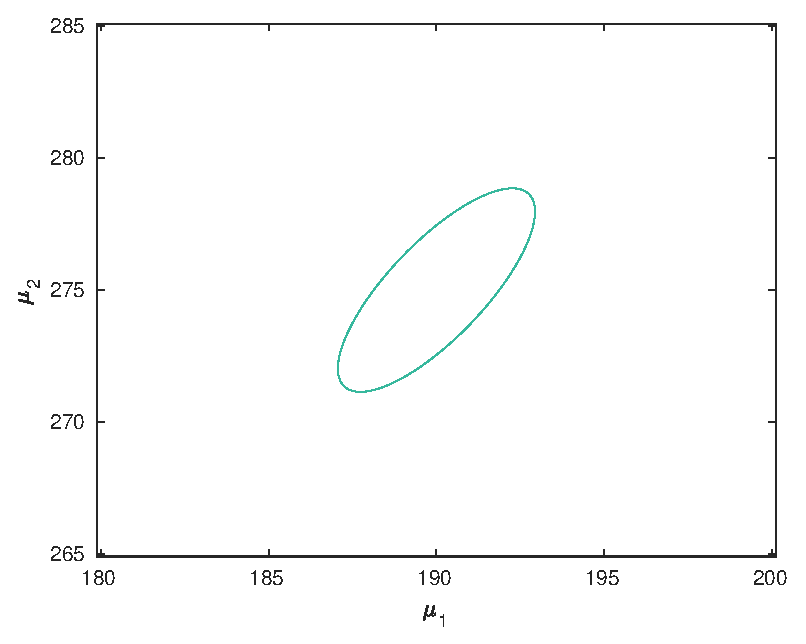
\includegraphics[width=5cm]{ellipse-ex1}
  \caption{The confidence ellipse around ${\bf \mu}$.}
  \label{fig:ex1-ellipse}
\end{figure}

\subsection*{(c)}
\label{sec:c}

Using $a_1 = (1,0)^T$ and $a_2 = (0,1)^T$, we find that the confidence
interval around $\mu_1$ is given by
\begin{equation*}
  \left(
    a \pm T_{1-\alpha} \sqrt{\frac{a_i^T S a_1i^T}{n}}
  \right), \quad i = 1,2,
\end{equation*}
with $T_{1-\alpha} = \frac{n-p}{p(n-1)}F_{1-\alpha}(p, n-p)$. Thus we
get the confidence intervals
\begin{align*}
  (184.7356&,\ 195.2644),\quad i = 1, \\
  (268.0801&,\ 281.9199),\quad i = 2.
\end{align*}

\subsection*{\texttt{matlab} code}
\lstinputlisting[style=matlab]{../ex1.m}

%%% Local Variables:
%%% mode: latex
%%% TeX-master: "examination"
%%% End:
